\documentclass[english]{article}



\usepackage{graphicx}
\usepackage{grffile}
\usepackage[T1]{fontenc}
\usepackage{babel}
\usepackage{float}
\usepackage{tabu}
\usepackage{ragged2e}
\usepackage{textcomp}
\usepackage{amstext}
\usepackage[final]{pdfpages}
\usepackage{caption}

\graphicspath{{Pictures/}}


\begin{document}

	
	\begin{figure}
		
\includegraphics[width=\linewidth]{up_logo.png}
	\end{figure}
	
	\begin{center}
	 \line(1,0){370}
	\\[0.2cm]
    {\scshape\Large Testing Report  \par}
	\vspace{0.1cm}
	\line(1,0){370}
	\\[0.8cm]
	
	 {\scshape\Large Broadsword Access \par}
	\vspace{0.9cm}
	
	\begin{tabu} to \textwidth { X[l] X[l]}
		\hline
		\textbf{Surname, First Name  }	& \textbf{Student Number}	\\ \hline \hline
		Pennels 	Keaton   & u14373018	\\ \hline
		Mpofu	Munyaradzi   &15071830		\\ \hline
		Cilliers	Joshua   &14267196		\\ \hline
		Walsh     Brent    &15300201		\\ \hline
		Groutsch	Stephanie    &14293324		\\ \hline
		Schouwstra	Rikard    &15012299		\\ \hline
		\hline
	\end{tabu}
	
	\end{center}
	
	
	\pagenumbering{gobble}
	\newpage
	\tableofcontents

	\pagenumbering{arabic}
	\newpage
	
	\section{Introduction}

				This chapter of the document aims to present the findings of the indepth testing done on the Gladios instance of the NavUP application. A test model was used for the various specifications of the core functions and innovations implemented.

		\subsection{Definitions, Acronyms, and Abbreviations}\label{subsec:daa}
			\begin{table}[h!]
				\centering
				\caption{Table of Definitions, Acronyms, and Abbreviations used in this document}
				\label{tab: Table 1}
				\begin{tabular}{| m{4cm} | m{12cm} |}
					\hline
					\textbf{Term} & \textbf{Definition} \\
					\hline
					\hline

		
					\hline
					

				\end{tabular}
			\end{table}


		\subsection{Overview}
			The remainder of this document will consist the test model used during testing, to functional requirements tested as well as the non-functional requirements tested.\\


	https://github.com/KeatonPennels/COS-301-Broadsword-Access
		  
	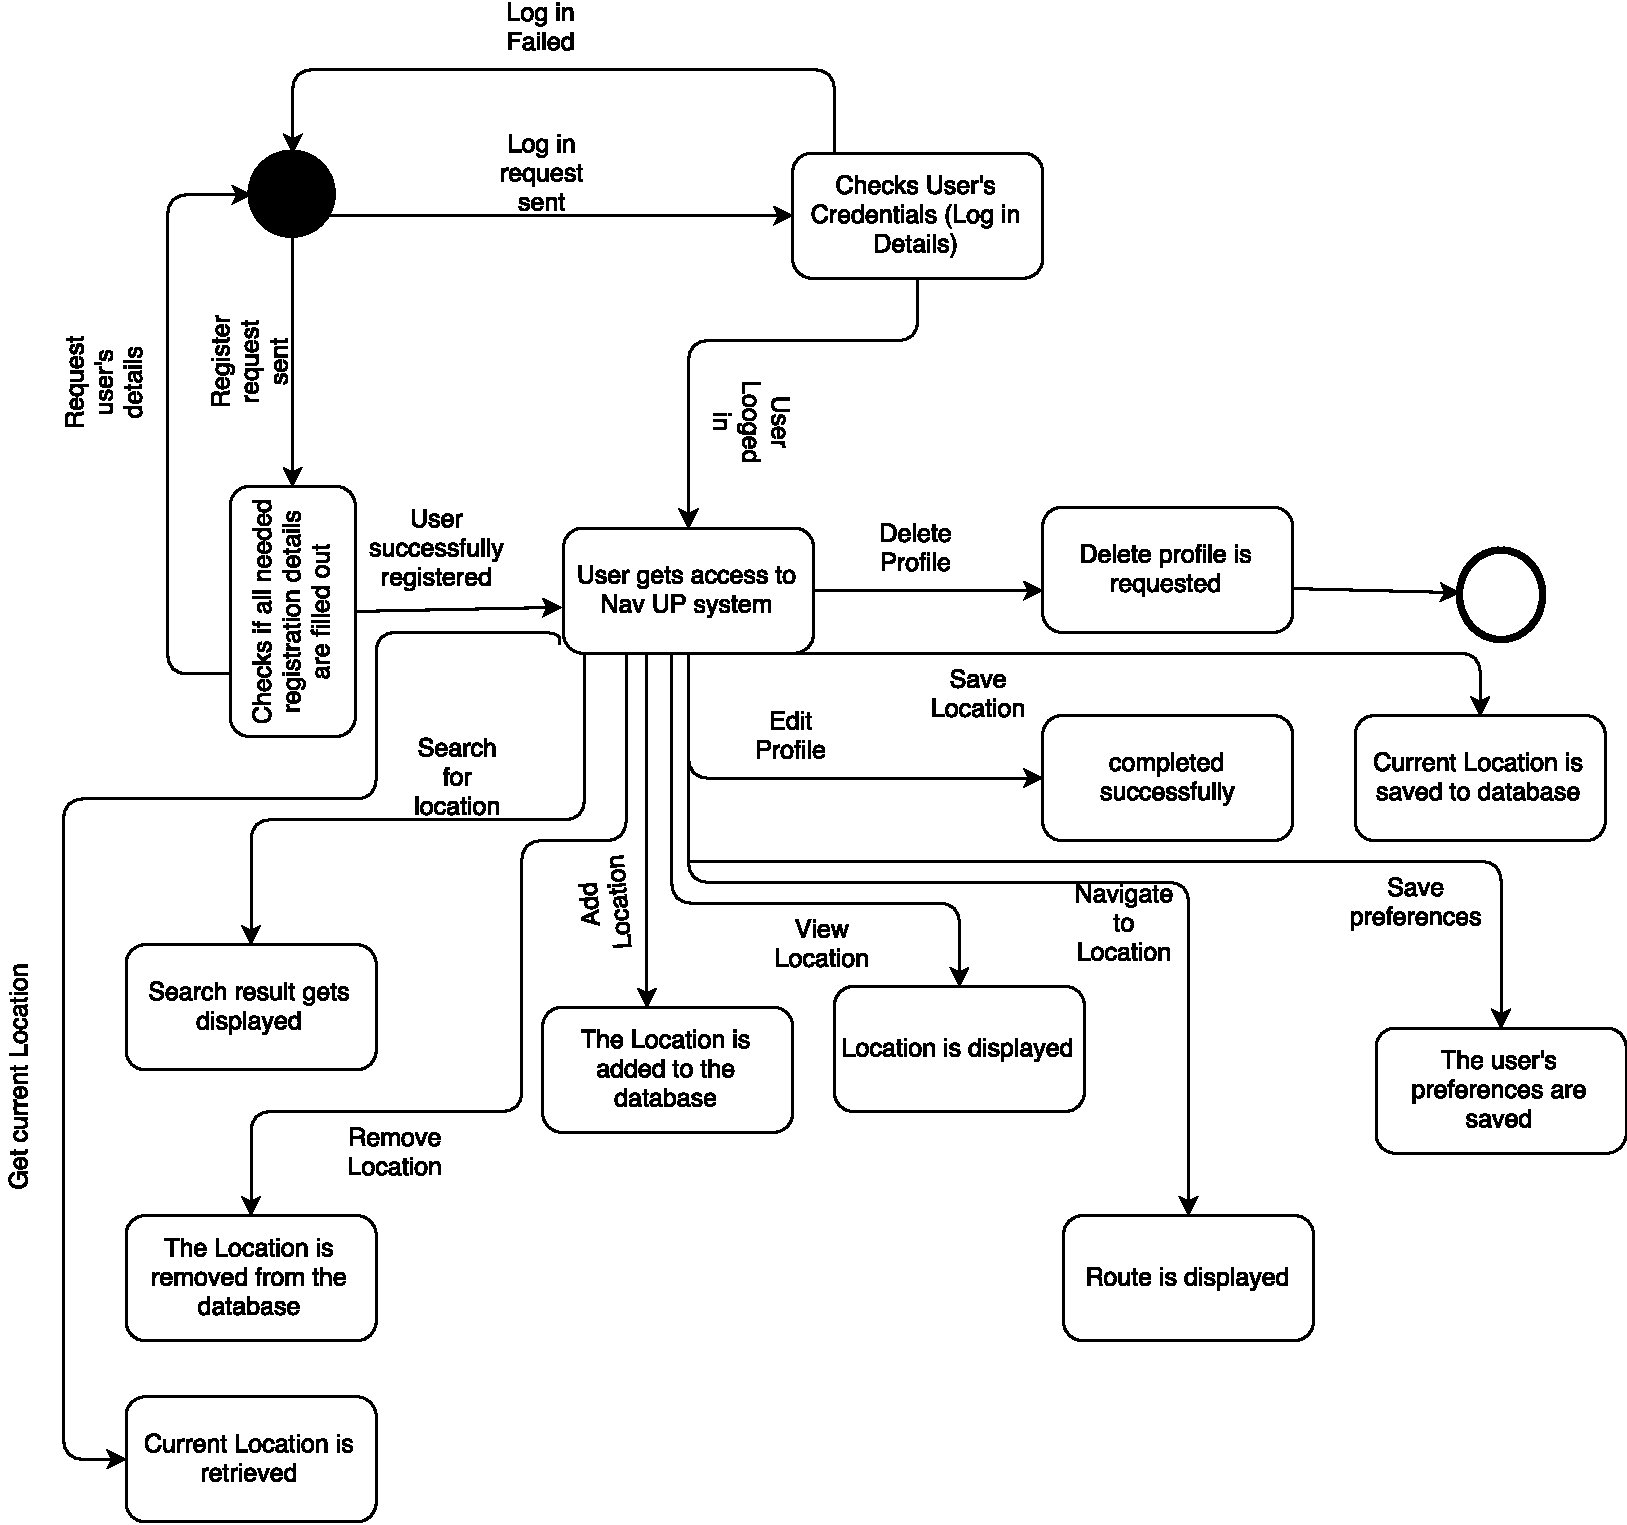
\includepdf[scale=0.8,pages=-,pagecommand=\section{Test Model}]{Test_Model.pdf}

		\clearpage
	\section{List of Service Contracts Tested}
	NavUP is currently envisioned as a native mobile application that serves to navigate users around the Hatfield campus of the University of Pretoria. This application will be utilised by students, staff and visitors to the Hatfield campus in order to find their way around.\\
	\subsection{Users}
\subsubsection{User Registration}

\begin{figure}[H]
\centering
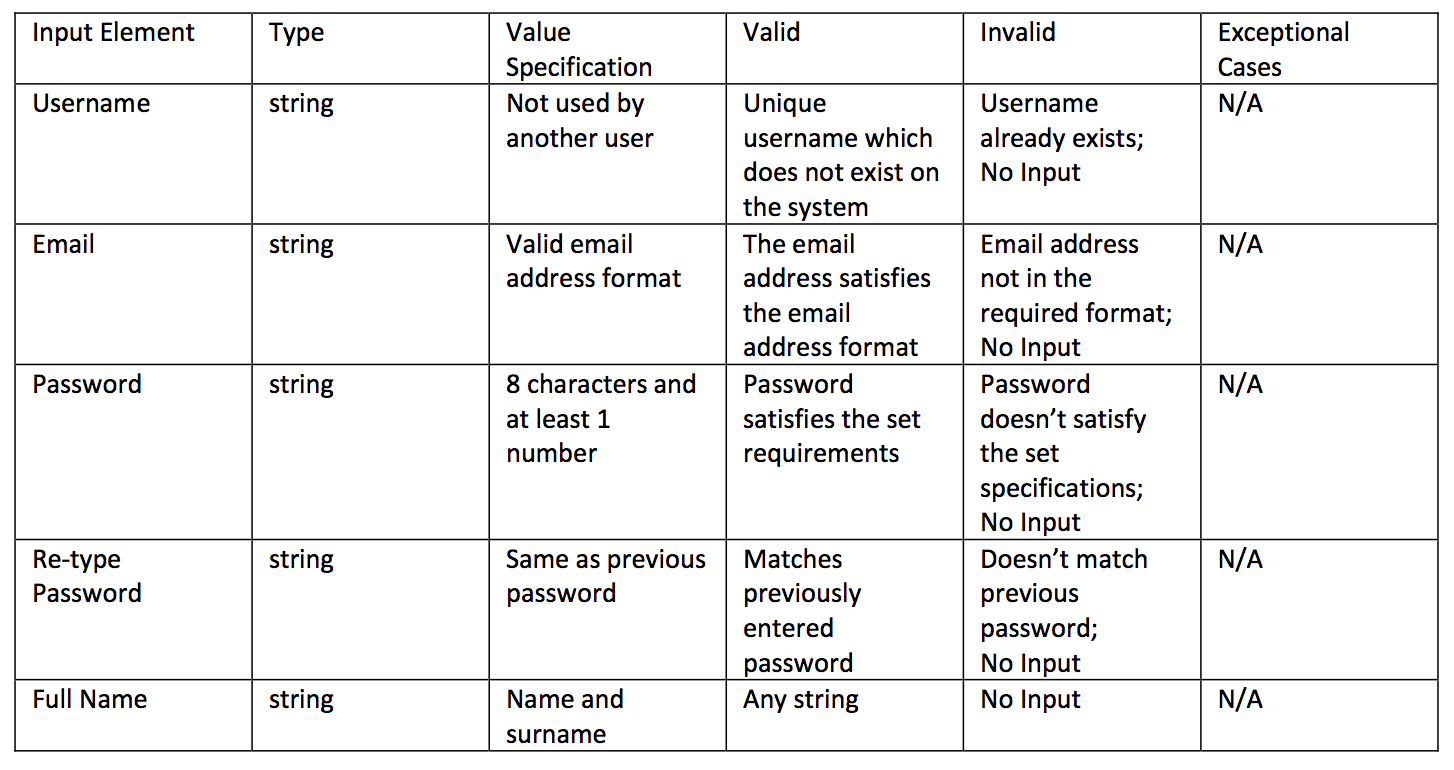
\includegraphics[width=1.0\textwidth]{Input_Values_Required}
\caption{Input Values Required}
\end{figure}
\begin{figure}[H]
\centering
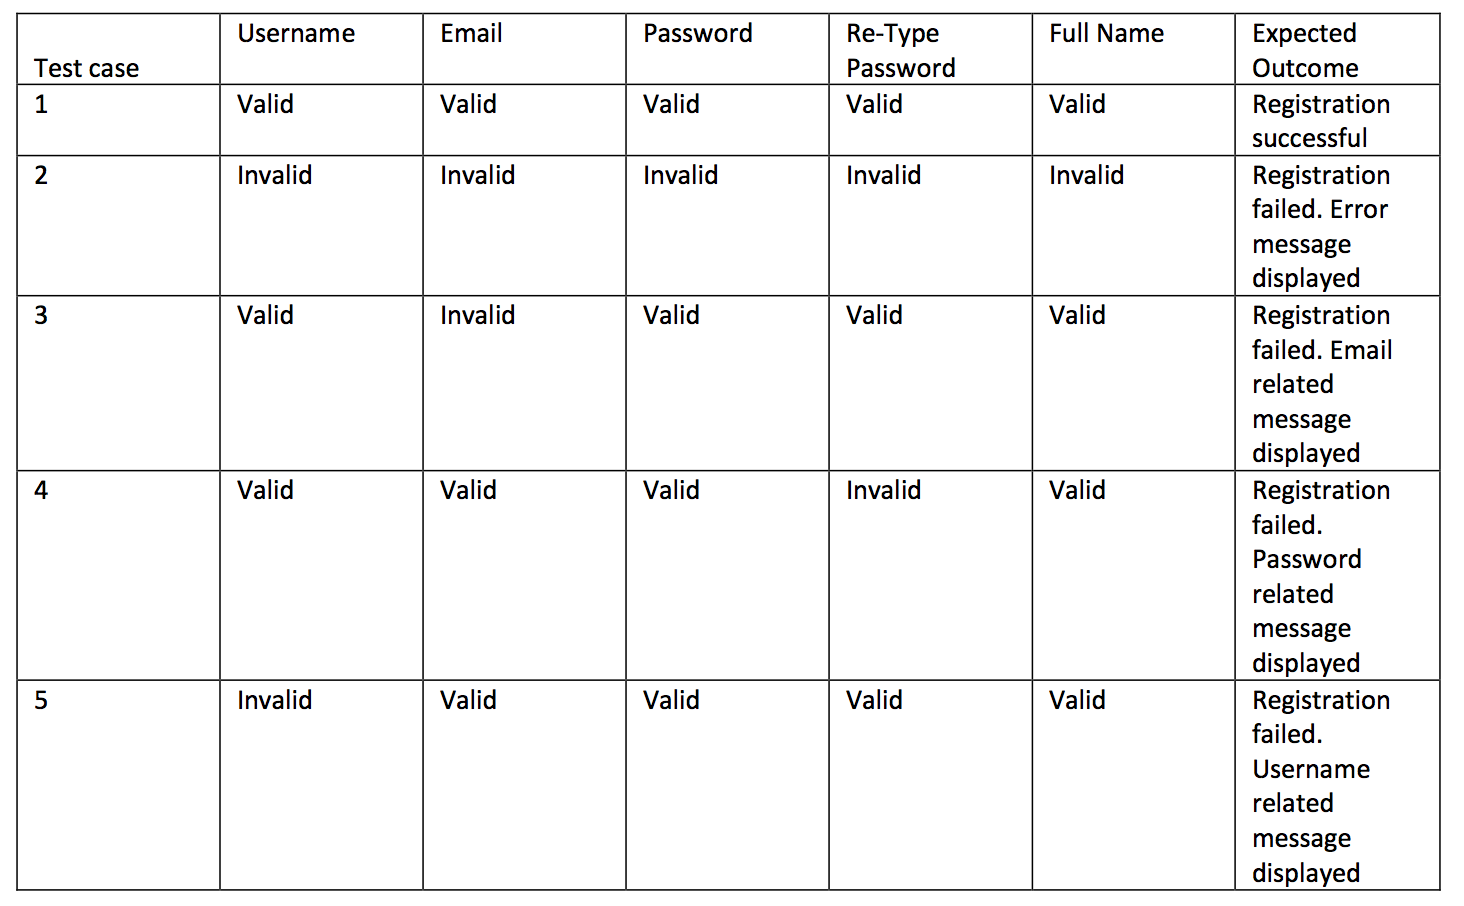
\includegraphics[width=1.0\textwidth]{Test_Cases}
\caption{Test Cases}
\end{figure}
\begin{figure}[H]
\centering
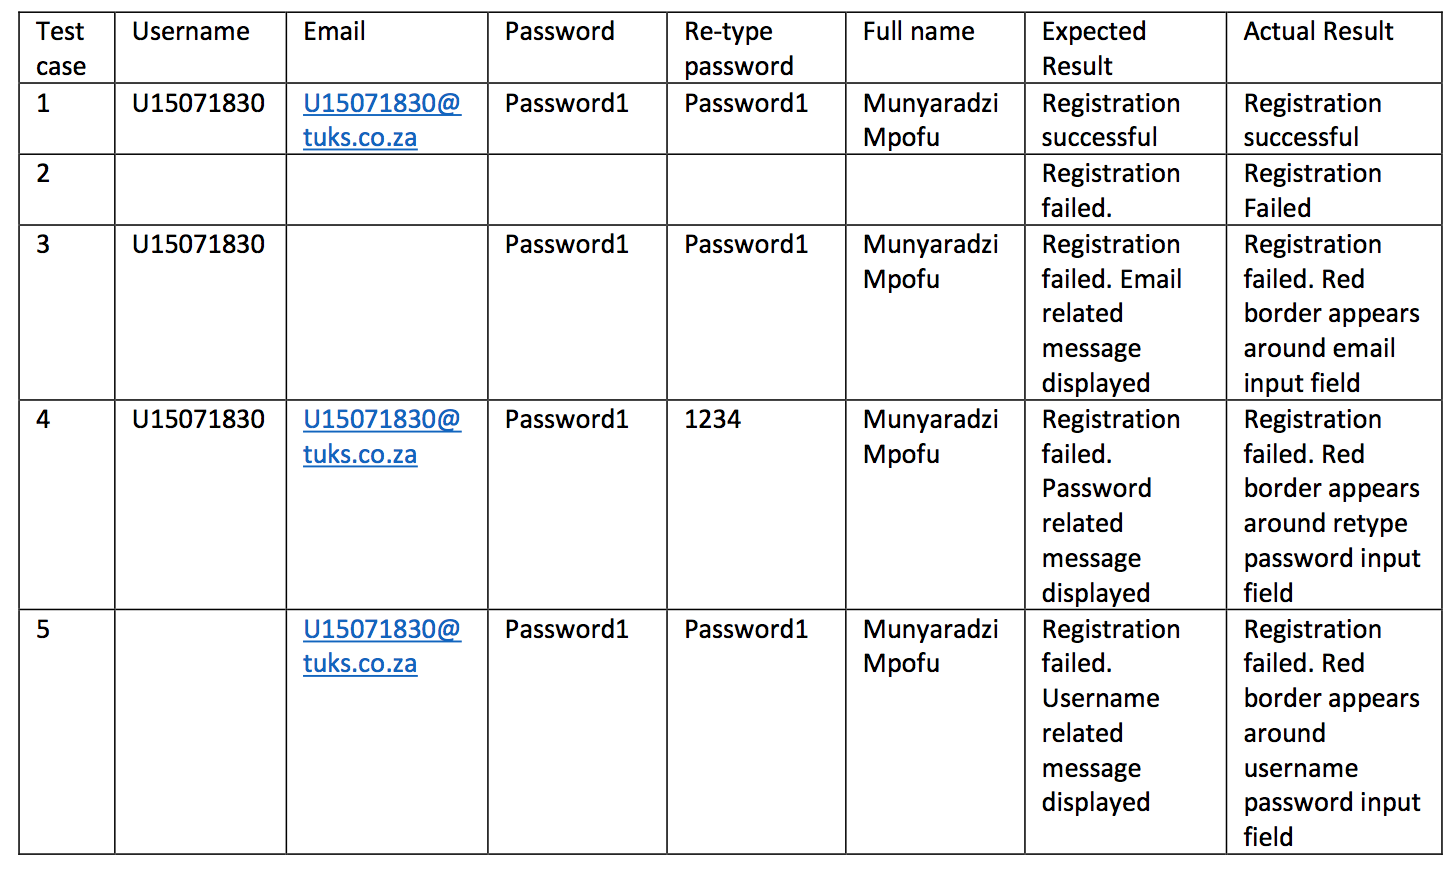
\includegraphics[width=1.0\textwidth]{Use_Case_Based_Testing}
\caption{Use Case Based Testing}
\end{figure}

\textbf{\underline{Test Case 1}}\newline
\textbf{Action:} Fill out all of the user registration details with correct data\newline
\textbf{Expected Result:} The registration is a success\newline
\textbf{Actual Result:} The registration was a success. A message is displayed to the user to indicate it was a success and the user is navigated back to the sign in page\newline

\textbf{\underline{Test Case 2}}\newline
\textbf{Action:} All registration input fields are left blank\newline
\textbf{Expected Result:} The registration is unsuccessful\newline
\textbf{Actual Result:} The registration was not successful; the input boxes had a red outline to indicate that the data needed to be filled in\newline
\textbf{Possible improvements:} Feedback in the form of text could have been given to indicate that the data needs to be filled in before a successful registration can be achieved\newline

\textbf{\underline{Test Case 3}}\newline
\textbf{Action:} An incorrect email address is entered\newline
\textbf{Expected Result:} The registration is unsuccessful\newline
\textbf{Actual Result:} The registration was a success\newline
\textbf{Possible improvements:} The application should check if the users email address actually exists before allowing users to register with it\newline

\textbf{\underline{Test Case 4}}\newline
\textbf{Action:} Register using two different passwords\newline
\textbf{Expected Result:} The registration is unsuccessful\newline
\textbf{Actual Result:} The registration was not successful, the password input boxes have a red border to indicate there was a problem \newline
\textbf{Possible improvements:} More feedback could be given. For example, a message saying that the passwords are not the same could be displayed. This would help the user as there could be other issues with the password such as it not being long enough or the password is not successful since it may need capital letters or characters.\newline

\textbf{\underline{Test Case 5}}\newline
\textbf{Action:} Register using two different email addresses\newline
\textbf{Expected Result:} The registration is unsuccessful\newline
\textbf{Actual Result:} The registration was not a success, the email input boxes have a red border around them.\newline
\textbf{Possible improvements:} More feedback could be given as to what the problem with the email addresses was.\newline

\textbf{\underline{Test Case 6}}\newline
\textbf{Action:} Register more than one user with the same username\newline
\textbf{Expected Result:} The registration is unsuccessful\newline
\textbf{Actual Result:} The registration was a success\newline
\textbf{Possible improvements:} More should be done in order to ensure that only users with unique usernames are allowed to register.\newline

\textbf{\underline{Test Case 7}}\newline
\textbf{Action:} Register more than one user with the same email address\newline
\textbf{Expected Result:} The registration is unsuccessful\newline
\textbf{Actual Result:} The registration was a success\newline
\textbf{Possible improvements:} The system should ensure that users are not registered to the application if their given email address is already been used by another user. This is important since email addresses are used to sign into the application.\newline\newline

\textbf{\underline{Total Mark: 4.5/10}}\newline
\textbf{Additional Comments:} Since almost half of the registration tests failed, the awarded mark out of ten was reduced to five and a half. This mark was then reduced by one since other improvements such as more feedback could be added in order to improve the registration process. \newline

\subsubsection{User Login}

\begin{figure}[H]
\centering
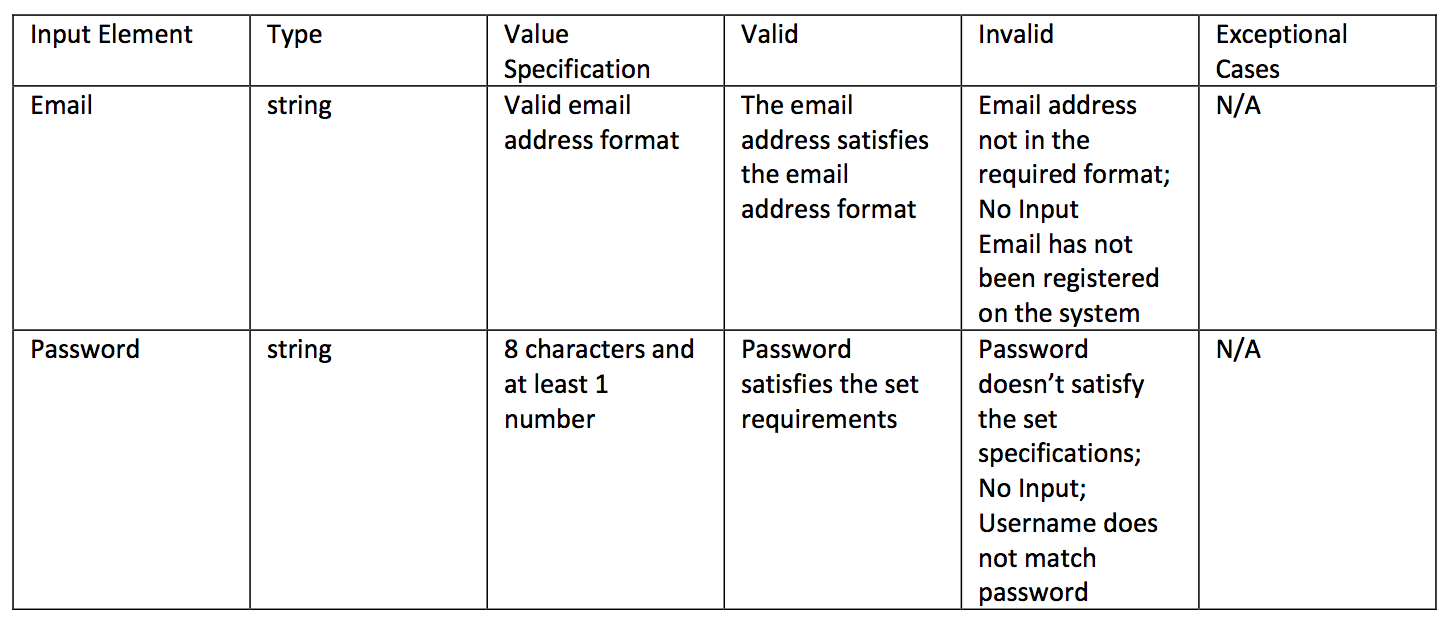
\includegraphics[width=1.0\textwidth]{userlogin_input_values_required}
\caption{Input Values Required}
\end{figure}

\begin{figure}[H]
\centering
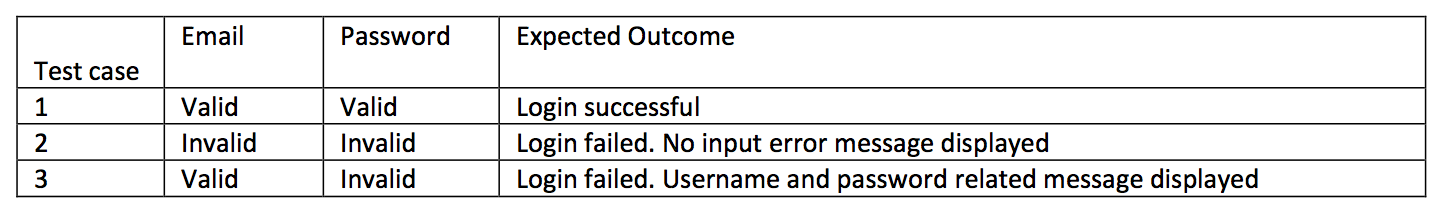
\includegraphics[width=1.0\textwidth]{userlogin_test_cases}
\caption{Test Cases}
\end{figure}

\begin{figure}[H]
\centering
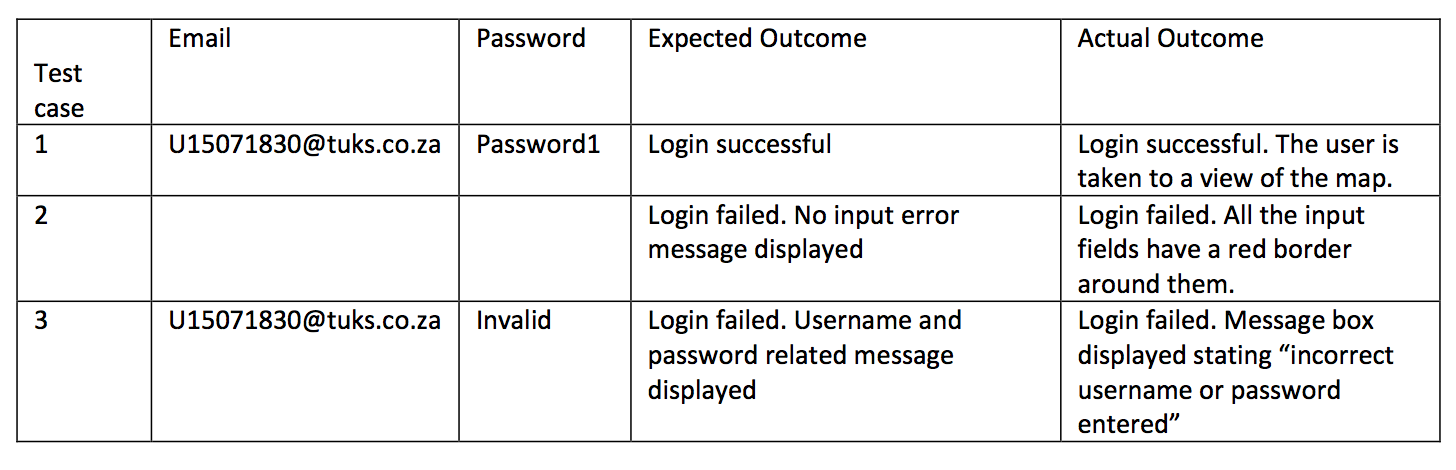
\includegraphics[width=1.0\textwidth]{userlogin_use_case_based_testing}
\caption{Use Case Based Testing}
\end{figure}

\textbf{\underline{Test Case 1}}\newline
\textbf{Action:} Fill out all of the user login details with correct data\newline
\textbf{Expected Result:} The user will be logged in successfully\newline
\textbf{Actual Result:} The login was a success; a message is displayed to the user that they have logged in successfully\newline
\textbf{Possible Improvements:} Instead of the application taking the user to the navigation page once they have logged in, they could instead be taken to a homepage. \newline

\textbf{\underline{Test Case 2}}\newline
\textbf{Action:} All login input fields are left blank\newline
\textbf{Expected Result:} The login is successful\newline
\textbf{Actual Result:} The login was not a success, the input boxes glow red to indicate that they should be filled in in order to login\newline
\textbf{Possible Improvements:} The user could also be notified by means of an alert which indicates why the login was unsuccessful\newline

\textbf{\underline{Test Case 3}}\newline
\textbf{Action:} Fill out the user login details with a correct username and an incorrect password\newline
\textbf{Expected Result:} The login is not successful\newline
\textbf{Actual Result:} The login was not a success, a message is displayed which states that either the email address or password were incorrect\newline

\textbf{\underline{Total Mark: 9/10}}\newline
\textbf{Additional Comments:} Since the actual results of all there test cases were the same as the expected results, the sign in should be awarded full marks. However, since the sign in can still be improved by giving the user more feedback when data is left blank, only 9/10 was awarded as there is still room for improvement.\newline

\subsubsection{Edit Profile}

\begin{figure}[H]
\centering
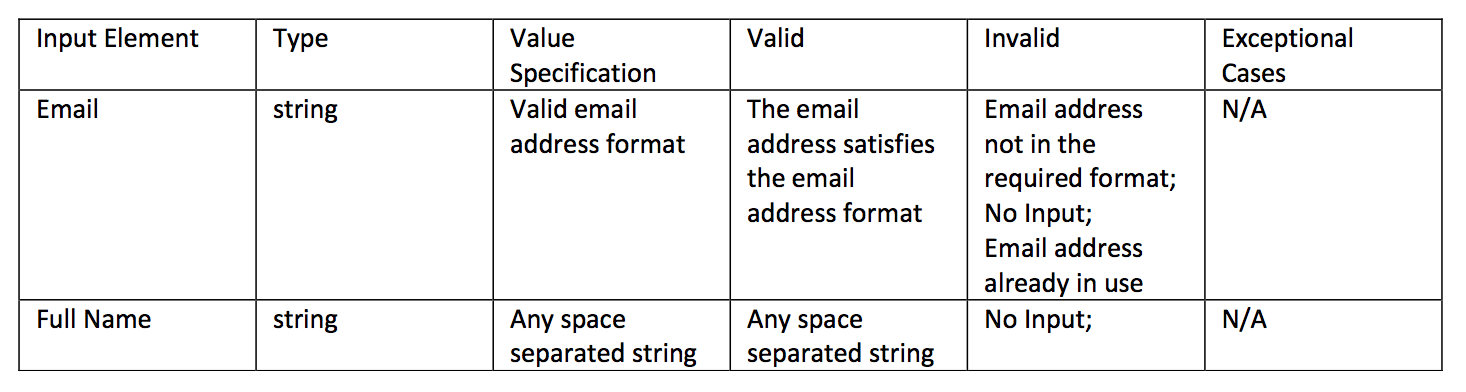
\includegraphics[width=1.0\textwidth]{editprofile_input_values_required}
\caption{Input Values Required}
\end{figure}

\begin{figure}[H]
\centering
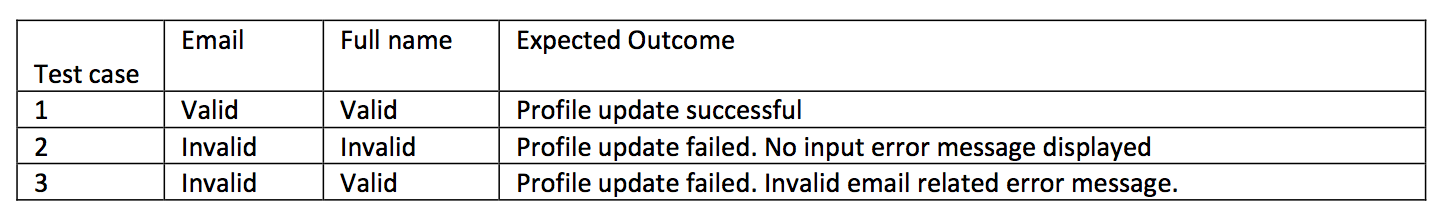
\includegraphics[width=1.0\textwidth]{editprofile_test_cases}
\caption{Test Cases}
\end{figure}

\begin{figure}[H]
\centering
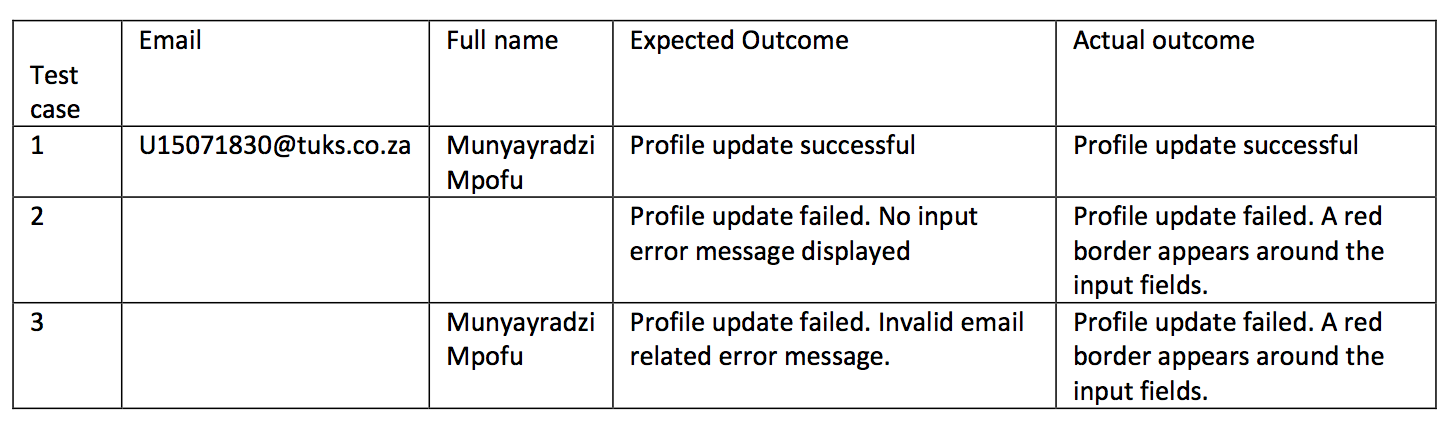
\includegraphics[width=1.0\textwidth]{use_case_based_testing_editprofile}
\caption{Use Case Based Testing}
\end{figure}

\textbf{\underline{Test Case 1}}\newline
\textbf{Action:} Update the user details and fill out all required input fields\newline
\textbf{Expected Result:} The profile update is successful\newline
\textbf{Actual Result:} The profile update is successful and the user is notified of the successful profile update.\newline
\textbf{Possible Improvements:} Once the profile has been updated, the application remains on the update profile screen. As a possible improvement, the application could navigate back to the menu instead.\newline

\textbf{\underline{Test Case 2}}\newline
\textbf{Action:} Update the user details and omit the details in one of the required input fields\newline
\textbf{Expected Result:} The profile update process is not completed.\newline
\textbf{Actual Result:} Upon clicking the "Update profile" button, a red border appears around the empty input field, and the profile update fails.\newline
\textbf{Possible Improvements:} A possible improvement would be to notify the current user by means of an alert indicating to them why the profile update failed.\newline

\textbf{\underline{Test Case 3}}\newline
\textbf{Action:} Update the user details with an invalid email address\newline
\textbf{Expected Result:} The profile update process is not completed.\newline
\textbf{Actual Result:} The update is a success even though the password is not valid\newline
\textbf{Possible Improvements:} The email address of the user should be validated \newline

\textbf{\underline{Total Mark: 5/10}}\newline
\textbf{Additional Comments:} The mark awarded for this module is 5/10 since the process of updating one’s profile was not a completely uniform process. This is mainly because the user has to navigate to a different page if they wish to update their password. Marks were also lost since one of the test cases failed. A possible improvement could be to add an input field to the “Edit Profile” page for the user to change their password. \newline

\subsubsection{Delete Profile}
N/A

\subsection{GIS (GIS Management)}

\subsubsection{View GIS Data}
\textbf{\underline{Test Case 1}}\newline
\textbf{Action:} The admin user presses the "Manage GIS" button\newline
\textbf{Expected Result:} The application displays an interface for the admin user to manage locations.\newline
\textbf{Actual Result:} The application displays a list of location names. It is assumed that this is a representation of GIS objects.\newline
\textbf{Possible Improvements:} The list of GIS locations displayed could also include the GPS coordinates of the location to the admin user.\newline

\textbf{\underline{Total Mark: 2/10}}\newline
\textbf{Additional Comments:} The application is intended to display an interface which an admin user can use to manage GIS locations, but instead it only provides a list of locations and no options to make any changes to these objects. \newline

\subsubsection{Add GIS Data}
N/A

\subsubsection{Edit GIS Data}
N/A

\subsubsection{Remove GIS Data}
N/A

\subsection{Points of Interest (Location Access)}

\subsubsection{Search Location}
\textbf{\underline{Test Case 1}}\newline
\textbf{Action:} The search icon is pressed with the intent of searching for a location on the map\newline
\textbf{Expected Result:} The application displays an input field in which the user can enter a location name and search for it\newline
\textbf{Actual Result:} The application displays a list of location names.\newline
\textbf{Possible Improvements:} The application could offer a search bar which the user can use to search for a specific location.\newline

\textbf{\underline{Total Mark: 2/10}}\newline
\textbf{Additional Comments:} The absence of a search bar when searching for a location could lead to a very inconvenient experience for the user, especially if the user has a large list of saved locations.\newline

\subsubsection{Save Location}
N/A

\subsubsection{Get Current Location}
\textbf{\underline{Test Case 1}}\newline
\textbf{Action:} The "Get Current Location" icon is pressed by the user.\newline
\textbf{Expected Result:} The application will mark the user's current location on the map\newline
\textbf{Actual Result:} The application marks a location on the map which is not the current user's location\newline
\textbf{Possible Improvements:} A possible improvement would be to mark the user's correct location on the map\newline

\textbf{\underline{Total Mark: 2/10}}\newline
\textbf{Additional Comments:} The application marks a location on the map, although this locations is not the correct location. This would lead to incorrect locations being saved, and could also affect the process of navigating from the users current location to another desired location.\newline


\subsection{Points of Interest (Location Management)}

\subsubsection{View Locations}
N/A
\subsubsection{Add location}
N/A
\subsubsection{Modify Location}
N/A
\subsubsection{Remove Location}
N/A

\subsection{Navigation}

\subsubsection{Navigate to Location}
N/A
\subsubsection{Save Preferences}
N/A

	\begin{figure}[H]
\centering
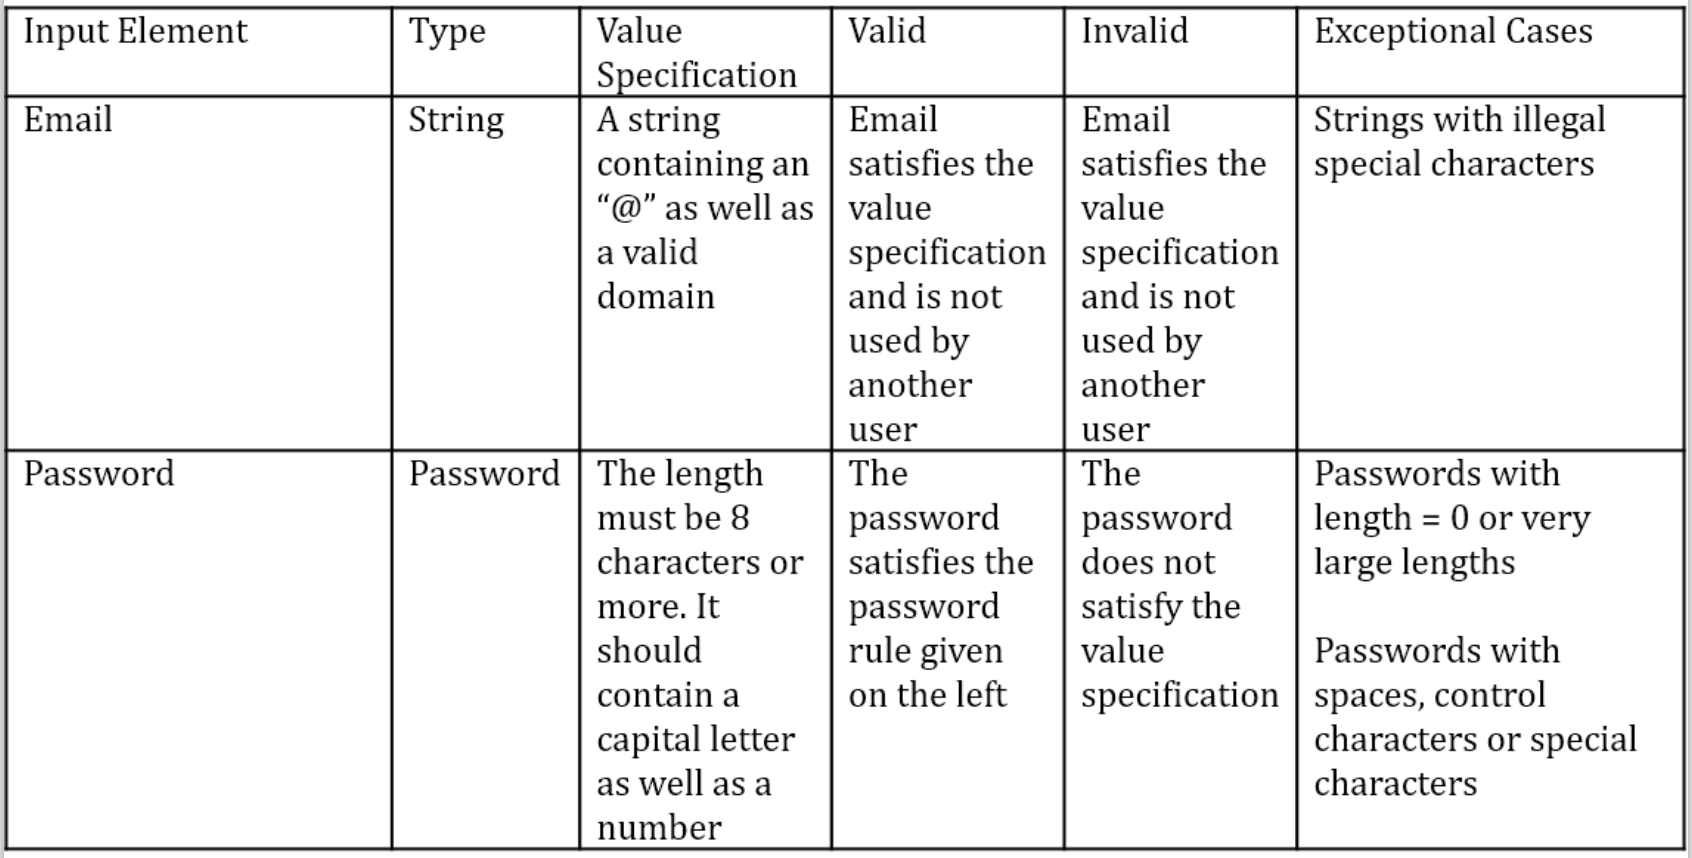
\includegraphics[width=1.0\textwidth]{registration_input_values_required}
\caption{Input Values Required}
\end{figure}

\begin{figure}[H]
\centering
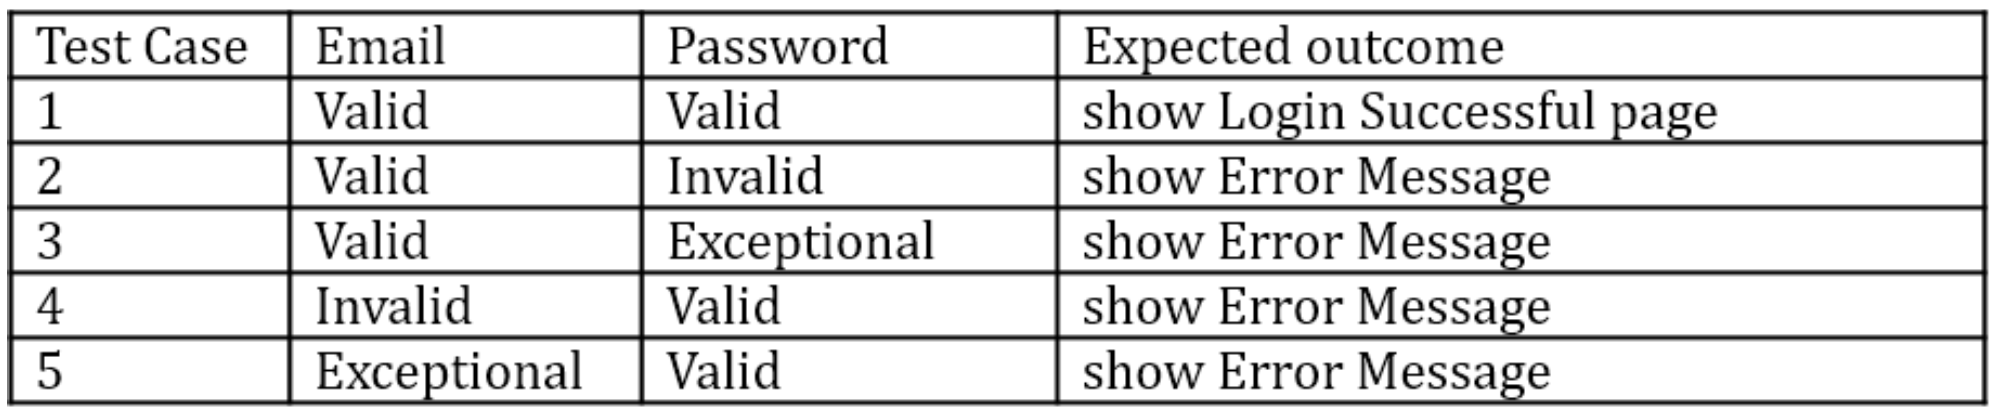
\includegraphics[width=1.0\textwidth]{registration_test_cases}
\caption{Test Cases}
\end{figure}

\begin{figure}[H]
\centering
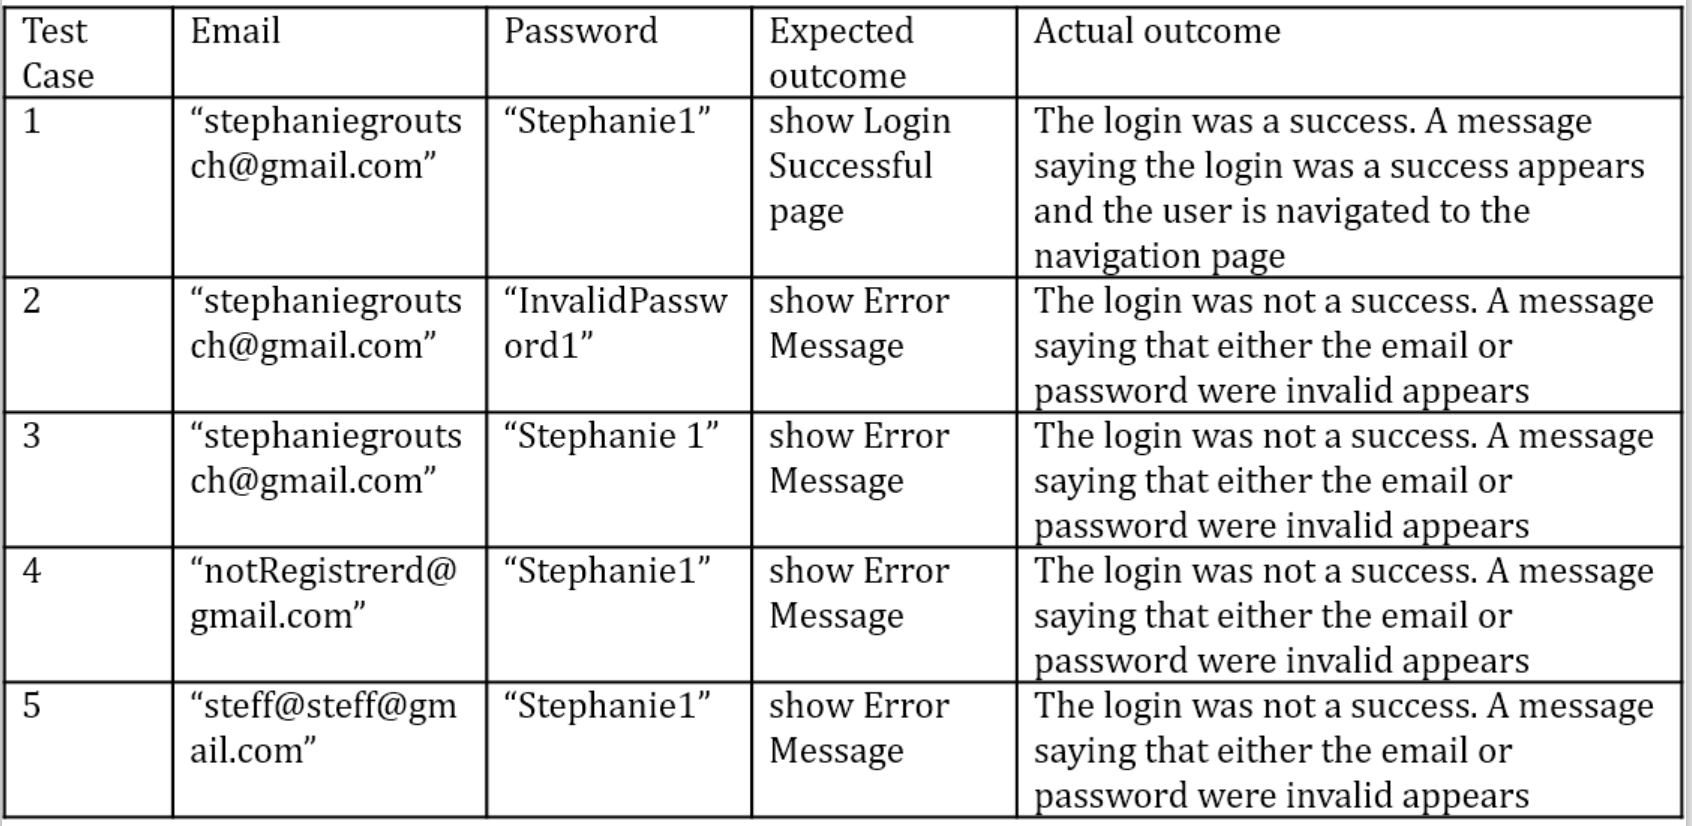
\includegraphics[width=1.0\textwidth]{registration_use_case_based_testing}
\caption{Use Case Based Testing}
\end{figure}
	
	\subsection{Registration}
Additional comments: 

Feedback in the form of text could have been given to indicate that data needs to be filled in before a successful registration can be achieved.

More should be done in order to ensure that only users with unique usernames are allowed to register

The system should ensure that users are not registered to the application if their given email address is already been used by another user. This is important since email addresses are used to sign into the application.

Since almost half of the registration tests failed, the awarded mark out of ten was reduced to five and a half. One mark was then subtracted from this mark since more feedback could have been given.

Mark awarded: 4.5/10

\subsection{Login:}

\begin{figure}[H]
\centering
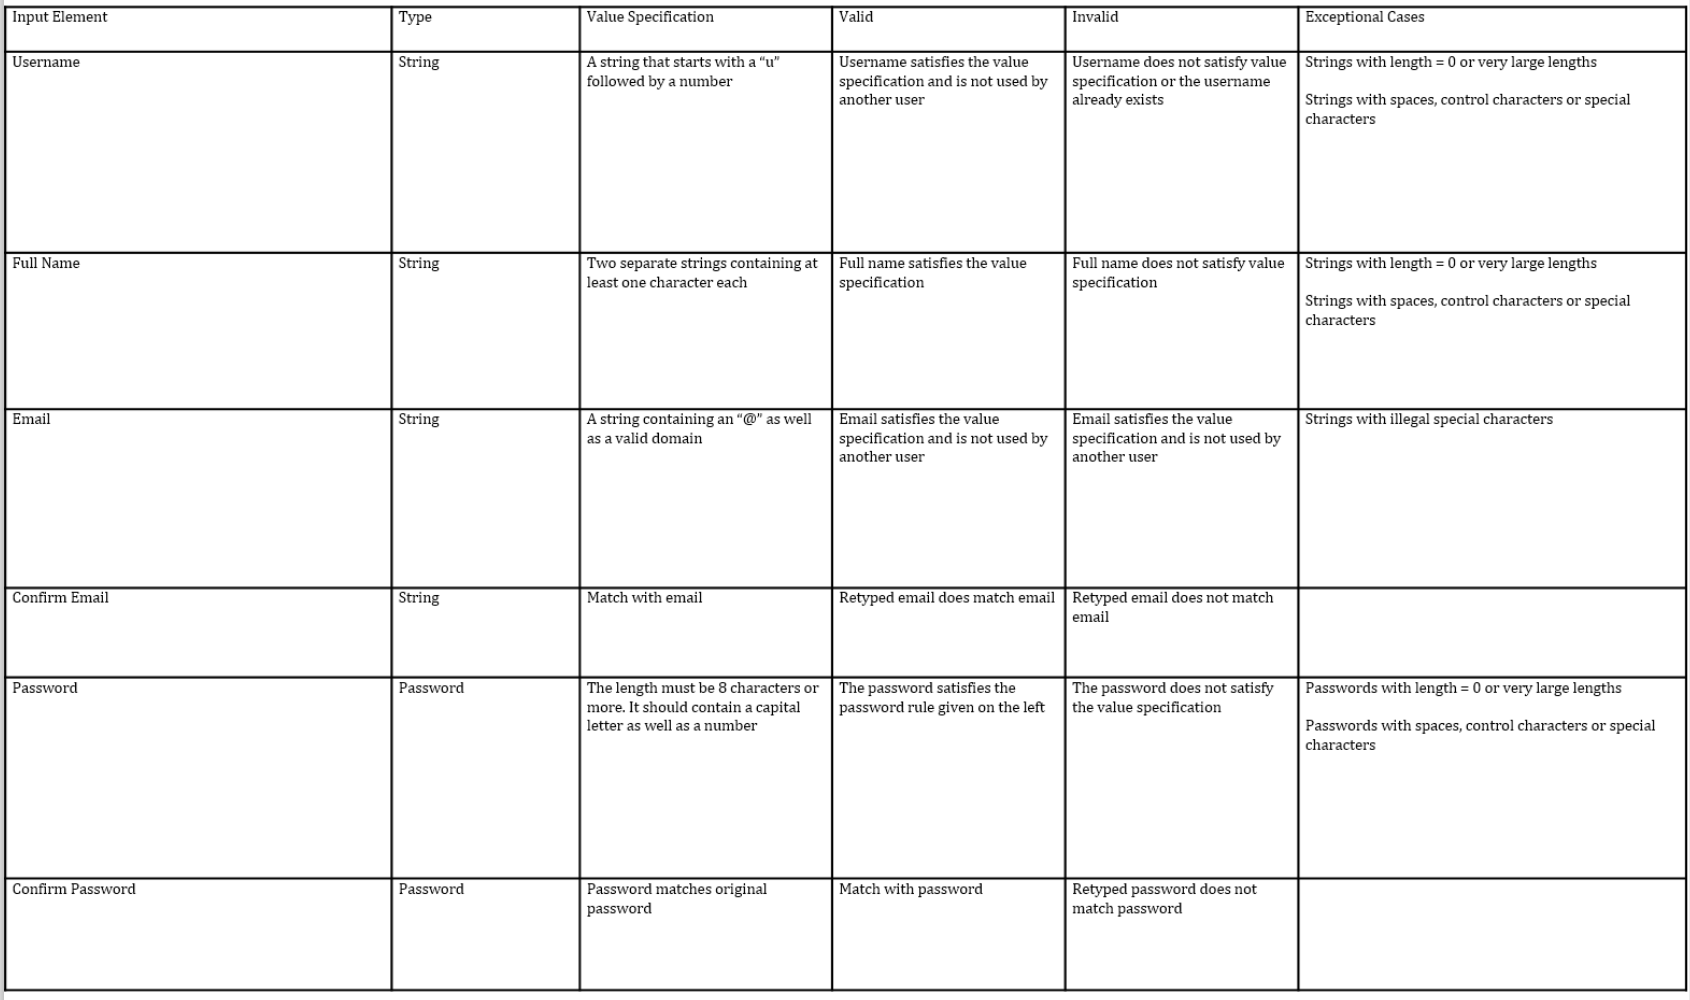
\includegraphics[width=1.0\textwidth]{login_input_values_required}
\caption{Input Values Required}
\end{figure}

\begin{figure}[H]
\centering
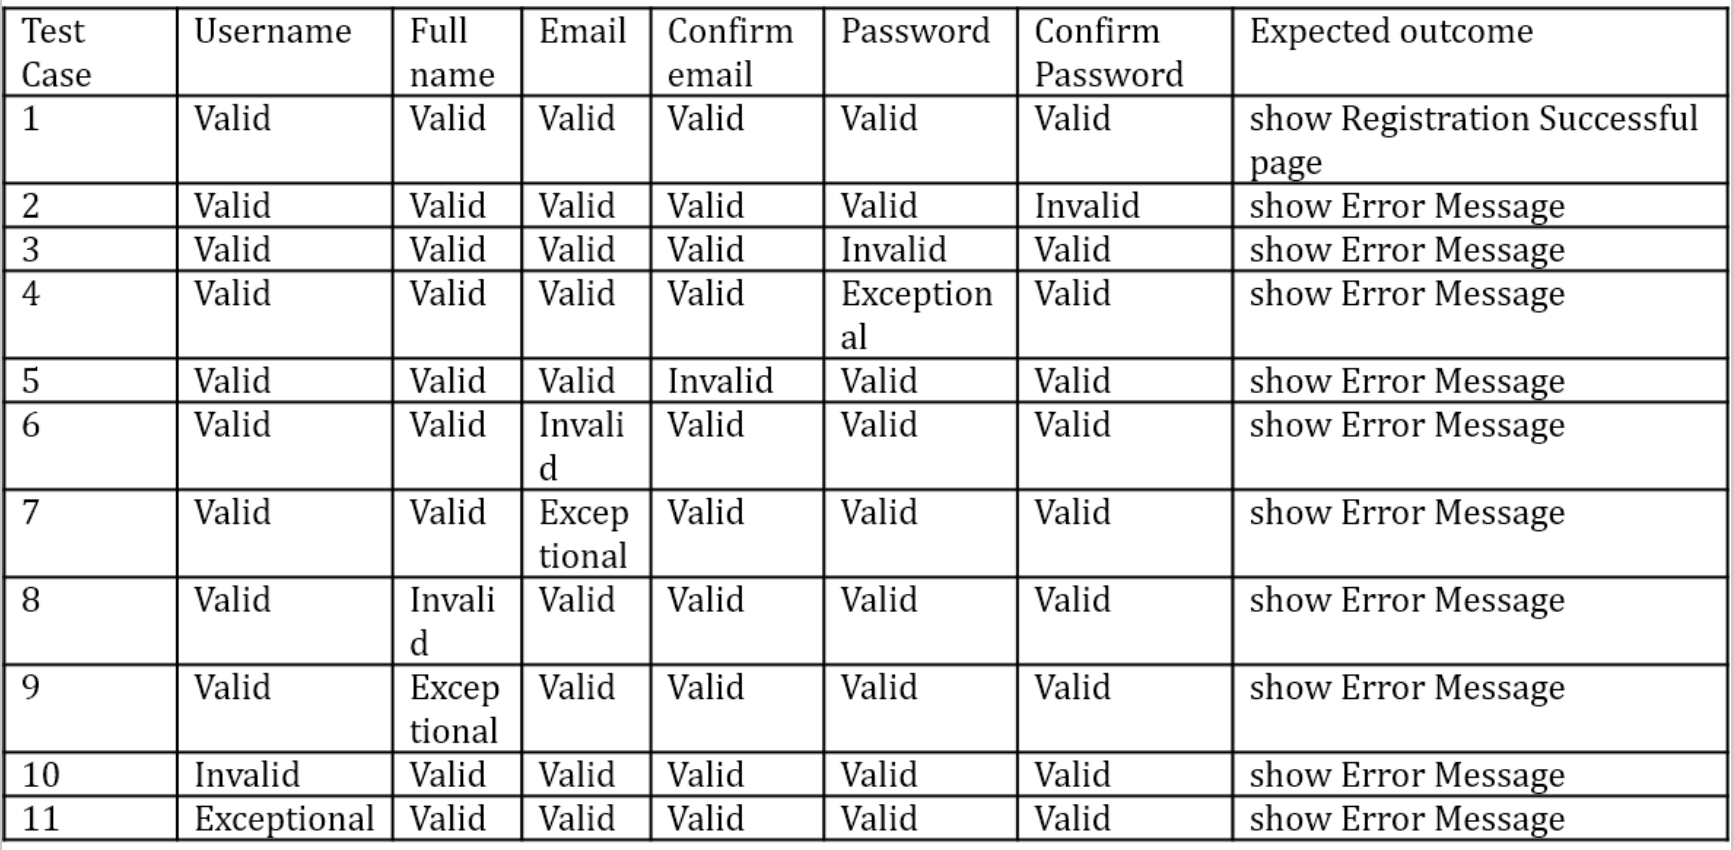
\includegraphics[width=1.0\textwidth]{login_test_cases}
\caption{Test Cases}
\end{figure}

\begin{figure}[H]
\centering
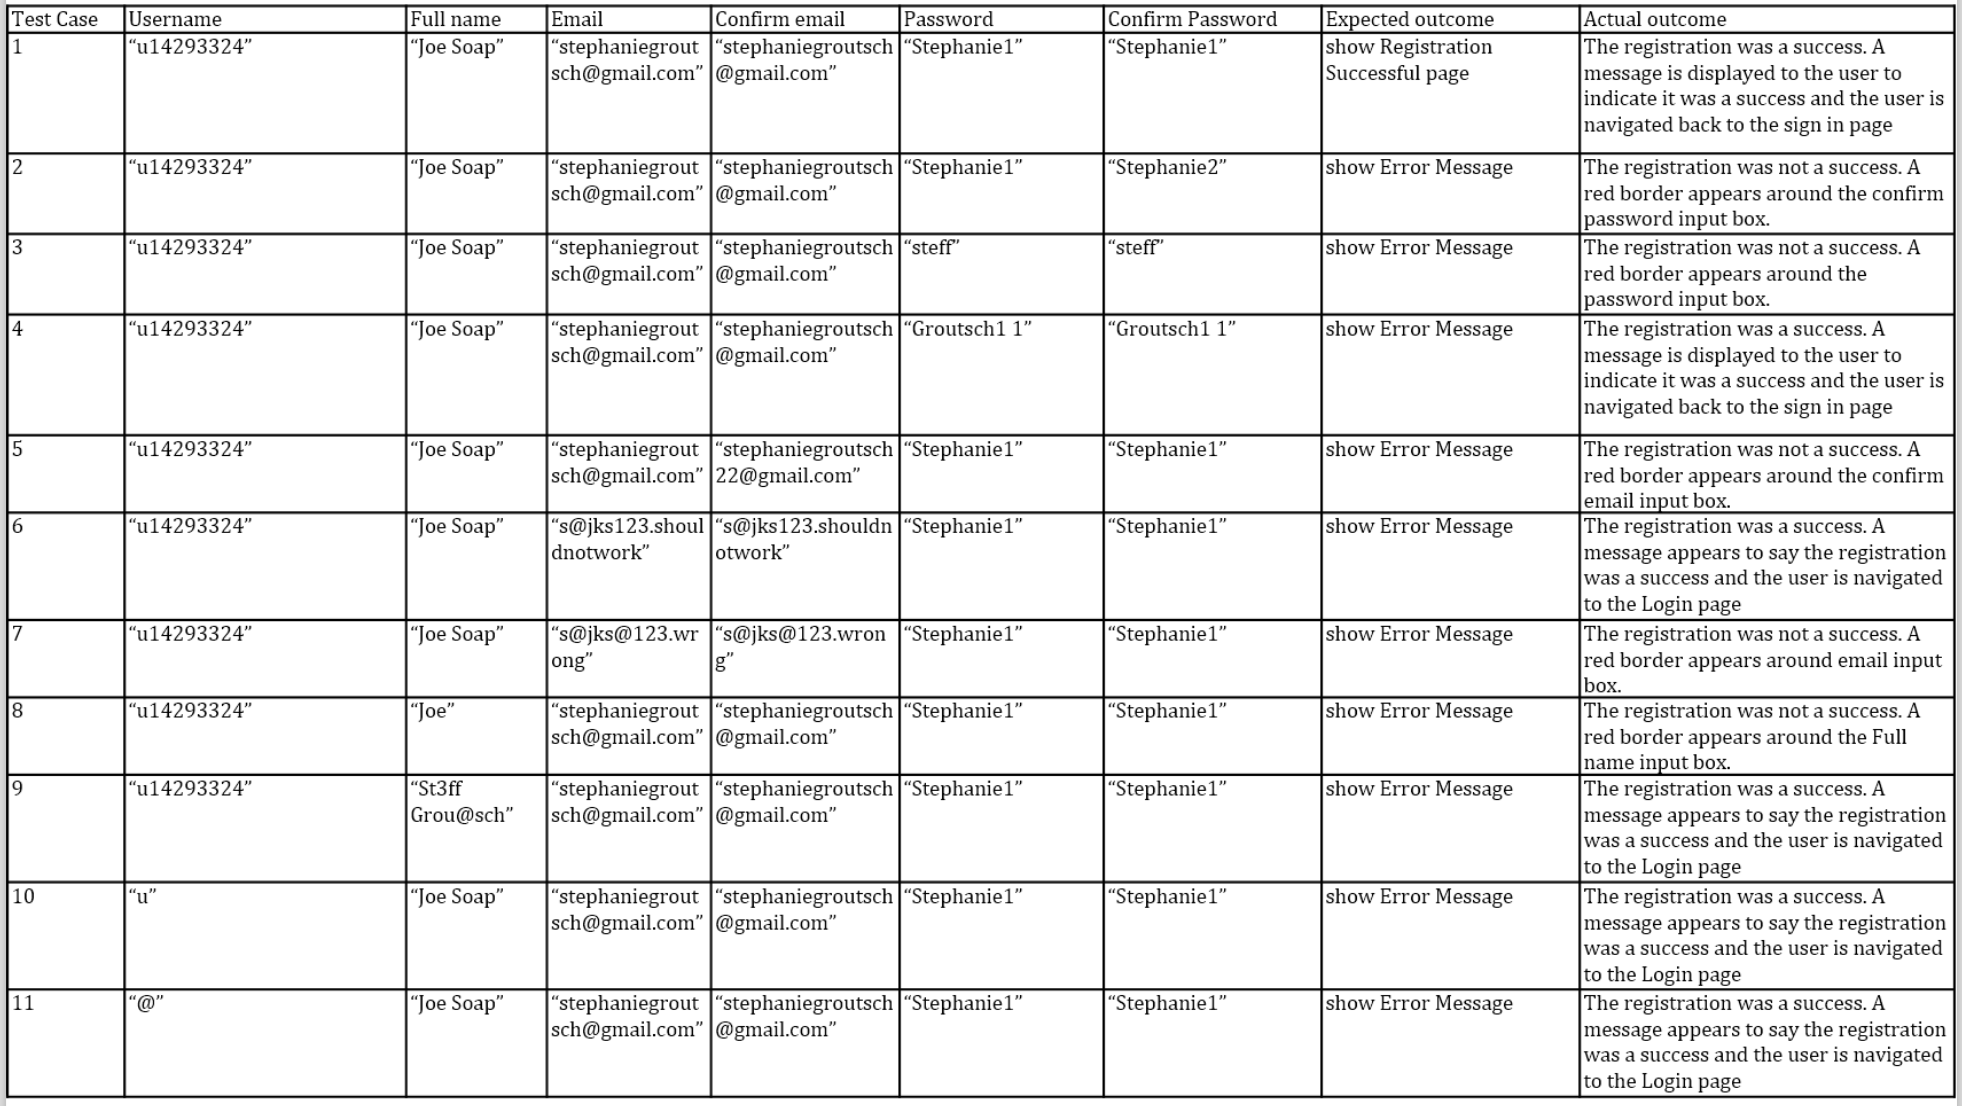
\includegraphics[width=1.0\textwidth]{login_use_case_based_testing}
\caption{Use Case Based Testing}
\end{figure}

Additional comments:

Instead of the application taking the user to the navigation page once they have logged in, they could instead be taken to a homepage. 

The sign in can still be improved by giving the user more feedback when data is left blank.

Since the actual results of all of the test cases were the same as the expected results, the sign in should be awarded full marks. However, since the sign in can still be improved by giving the user more feedback when data is left blank, only 9/10 was awarded as there is still room for improvement.

Mark awarded: 9/10

	\section{List of Functional Requirements Tested}
	This chapter aims to give an overview of the entire NavUP system. The system will be contextualised in order to demonstrate the basic functionality of the system as well as demonstrate how the system interacts with other systems. It will also describe the levels, or types, of users that will utilise the system and describe the functionality that is available to said user. At the end of this chapter, the constraints and assumptions for the system will be addressed.
	
	\begin{itemize}
		\item[$\bullet$] Create route to valid location
		\item[$\bullet$] Save routes
		\item[$\bullet$] Heat maps
		\item[$\bullet$] Current user location
		\item[$\bullet$] Save locations
		\item[$\bullet$] Search for locations
		\item[$\bullet$] Report protest action or emergency
		\item[$\bullet$] Create public event
		\item[$\bullet$] View all locations
		\item[$\bullet$] Request addition, removal, or modification of locations
		\item[$\bullet$] Register as student, staff, admin or guest
		\item[$\bullet$] Login
		\item[$\bullet$] Manage user accounts
		\item[$\bullet$] Add profile information
	\end{itemize}
	
	\section{List of Non-Functional Requirements Tested}
	
	\subsection{Performance requirements:}
\subsubsection{Performance:}
	\begin{itemize}
		\item[$\bullet$] Offline activities should have a response time of +/- 2 seconds (instantaneous) when responding to an activity, while online activities such as calculating routes should have a response time of +/- 2-4 seconds so that the users have an uninterrupted experience.
		\item[$\bullet$] It should also allow the integration of a variety of services.
	\end{itemize}

\subsubsection{Reliability:}
\begin{itemize}
\item[$\bullet$]The application should be reliable, in that it will provide the fastest route every time without fail and complete all other computations successfully. 
\item[$\bullet$]All activities should be completed with a 10% error allowance.
\item[$\bullet$]The application should provide accurate locations in a constantly changing environment.
\end{itemize}

\subsubsection{Security:}
\begin{itemize}
\item[$\bullet$]Data transmission should be securely transmitted without unauthorized access, or loss of information.
\end{itemize}

\subsection{Design Constraints:}

\begin{itemize}
\item[$\bullet$]The system should be accessible on smart devices, such as Android and iOS devices.
\item[$\bullet$] The system should not use GPS, but only the WiFi network.
\item[$\bullet$] The proposed system should be able to be integrated into the Computer Science Department's Web site.
\item[$\bullet$]The system should be a modular system, to reduce the dependencies in the system.
\item[$\bullet$]Software Fault Tolerance: If a malfunction cannot be avoided, then the software design should be constrained so that the system can recover without causing damage to the system.
\item[$\bullet$]The system should have an aesthetically pleasing and easy to use interface.
\item[$\bullet$]The system must be able to run on smart devices which has limited processing power, battery life and storage space. The system must thus use resources efficiently. 
\item[$\bullet$]The system needs to use open source technologies.
\end{itemize}	

\subsection{Software System Attributes:}

\begin{itemize}
\item[$\bullet$]Users should have the option to withdraw all information gathered by the system.

\item[$\bullet$]The system should be available online as well as offline.

\item[$\bullet$]The system should stay updated, to ensure reliable information. For instance the maps of campuses should be updated regularly.

\item[$\bullet$]The system should easily be updated, without complications.

\item[$\bullet$]The system should be managed efficiently, checking for problems regularly.

\item[$\bullet$]The system should be secure to prevent unauthorized modification or access of information.

\item[$\bullet$]The system should be user-friendly, the application should meet the requirements of the user by providing good access for disabled users, and resulting in a good overall user experience.
\end{itemize}	
	
	\section{Evaluation of Test Cases for Non-Functional Requirements}
	
\subsection{Security}\label{subsec:overall-security}
		    \textbf{\underline{Password Protection}}\newline
		    \textbf{Action:} Attempt to circumvent the password protection\newline
            \textbf{Expected Result:} The password protection should be secure and impervious to circumvention.\newline
            \textbf{Actual Result:} The password protection at the login screen is secure and doesn't allow users to login unless their password is correct. The Profile Management page however has a loophole when changing passwords though, in that it allows users to change passwords even if the password they enter into the Old Password field (for authentication) is incorrect.\newline
            \textbf{Possible Improvements:} The app should lock down the profile if the password is entered incorrectly too many times. The profile can then remain locked until an authentication email is sent to the user allowing them to unlock their profile. \newline
            \textbf{Mark:} 7/10\newline
            
            \textbf{\underline{SQL Injection}}\newline
		    \textbf{Action:} Attempt to inject SQL code into the database\newline
            \textbf{Expected Result:} The SQL injection should be blocked by escaping the special characters entered.\newline
            \textbf{Actual Result:} The SQL injection couldn't be tested because none of the data entered is persisted to a database. However, no code was found to sanitize harmful characters from user input before passing it to the user module. \newline
            \textbf{Possible Improvements:} The app could escape characters before passing it to the user module. \newline
            \textbf{Mark:} 2/10\newline

        \subsection{Stability}\label{subsec:overall-stability}
		    \textbf{\underline{Crash Testing}}\newline
		    \textbf{Action:} Attempt to crash the Access module through overloading input.\newline
            \textbf{Expected Result:} The app will remain running.\newline
            \textbf{Actual Result:} The app avoided crashing but was slowed down to an extent by the large amount of input.\newline
            \textbf{Possible Improvements:} The app should implement a character limit on input fields to fully guard against this issue.\newline
            \textbf{Mark:} 8/10\newline
            
        \subsection{Accessibility}\label{subsec:overall-accessibility}
		    \textbf{\underline{Support for disabilities with routes}}\newline
		    \textbf{Action:} Does the app provide an option for routes that are friendly to people with disabilities?\newline
            \textbf{Expected Result:} The app does provides such a feature with routes that avoid stairs and follow wheelchair-friendly routes.\newline
            \textbf{Actual Result:} The app does not provide such a feature.\newline
            \textbf{Mark:} N/A\newline
            
        \textbf{\underline{Support for colour-blindness}}\newline
		    \textbf{Action:} Does the app provide an option to present the User Interface in a manner that is colour-blind friendly?\newline
            \textbf{Expected Result:} The app has options for different kinds of colour-blindness.\newline
            \textbf{Actual Result:} The app doesn't provide support for different kinds of colour-blindness.\newline
            \textbf{Mark:} N/A\newline
	    
	    \subsection{Performance Testing}\label{subsec:overall-performance}
		A IPhone 6 with the below specifications were used in order to conduct the various performance testing \newline
		
		Specifications: Operating System – iOS 10.3 \newline
		  Chipset – Apple A8 \newline 
		 CPU – Dual Core 1.4 GHz \newline
		 RAM – 1GB DDR3  \newline
		 Storage – 32GB \newline
		 
		 The below table displays the performance statics gathered when running the NavUP application on the above device. The respective functionality was conducted 10 times and then an average of these cases were recorded in the Measure column. Recorded statistics were taken from the XCode debugging suite.
		 
		 \begin{table}[h!]
		 	\centering
		 	\caption{Table of collected data for Performance testing}
		 	\label{tab: Table 2}
		 	\begin{tabular}{111}
		 		\hline
		 		\textbf{Functionality} & \textbf{Description} & \textbf{Measurement}\\
		 		\hline
		 		\hline
		 		Application launch &	Time taken for home screen to load when application is opened & 1.42 seconds \\ 
		 		 & Initial memory usage when application is launched  & 118.3 MB  \\ 
		 	    &	Initial percentage of CPU used when application is launched &	0.8 \% \\
		 		 & Amount of data read when application is launched  &	40 KB \\
		 		 & Amount of data read when application is launched  &	300 KB \\
		 		 Registration  & 	Time taken to register a new user & 	0.7 seconds \\
		 		 &  Memory increase when new user is registered	 & 57.9 MB \\
		 		  & Amount of data written when new user is registered & 	1.2 MB \\
		 		 Profile Management & 	Time taken to update user details & 	0.2 seconds \\
		 		  & Memory increase when new user is registered	 & 10.6 MB \\
		 		  & Amount of data read when user profile is displayed & 	200 KB \\
		 		 &  Amount of data that was written when user details were updated & 	0.64 MB \\ 
		 		 
		 		
		 		
		 		
		 		\hline
		 		
		 		
		 	\end{tabular}
		 \end{table}
		
		\cleardoublepage
		
		We were unable to test the navigation with relation to performance as its functionality was not available to us. It was estimated that this would incorporated a large part of the applications performance requirements in terms of memory and CPU usage \newline
		
		\textbf{Mark =} 9/10 \newline
		Comment: The Gladios instance of the NavUP application performs well in terms of time taken for the application the execute user tasks. As this is the majority concern for all 3 user groups, this instance meets the requirements in terms of performance. The memory and CPU time required by the application is in general quite low which allows it to perform well even when other applications are running on a device. It would have been preferable if the performance requirements of navigation could have been tested in order to gauge how the application performs under general usage conditions.
		
		\subsection{Usability Testing}\label{subsec:usabilty}  
		
		The Gladios instance of NavUp usability testing was evaluated in terms of 3 key components: \textbf{Effectiveness} (Whether or not the user’s goal was achieved), \textbf{Efficiency} (Whether a user’s goal is achieved in a proficient manner) and \textbf{Aesthetics} (Whether the look and feel adhered and/or enhances applications purpose). \newline
		
		The user’s goals that were taken into consideration was that of all 3 different user groups of the NavUP application. All tasks were derived from the model Requirements Specifications. Upon completion of these 3 user groups interacting with the application, the following results were gathered. \newline
		
		\textbf{Effectiveness} – Guest and General users were able to carry out all tasks related to the core functionality required of the NavUP application whereas Admin users were not provided with required User and GIS administrative functionality. This was not seen as a major shortcoming in terms of effectiveness as the majority of administrative functionality would take place on the Web instance of the NavUP application. Tasks involving Add On functionality were sparsely implemented for all 3 user groups with only basic navigation functionality being provided to the users \newline
		
		\textbf{Efficiency} – The application provides a simple user interface and requires only basic touch, swipe and type interactions. The majority of functionality is reachable to the user within the range of 3 to 5 clicks/touches. Where the app lacks in efficiency is in two areas:  1) a call to action for the user upon launching the application was absent. The user was required to open a descriptionless menu tab in order being interaction and 2) providing guiding prompts to direct the user’s interaction with the application. Users were not informed of incorrect inputs and struggled when registering, logging in and searching.\newline
		
		\textbf{Aesthetics} – The user is presented with interface whose colour scheme is in conjunction with that of the University of Pretoria. This along with the structure of components within the application being similar to that of other popular navigation applications such as Google Maps and Waze Maps ensured that interactions would be intrinsically familiar to the user. All menus and search interactions were formatted consistently throughout the applications which prevented confusion and allowed for the user to become familiar with the user interface \newline
		
	\textbf{Mark =} 7/10 \newline
	
		Comment:  All three user groups have access to almost all of the core functionality and some of the add on functionality which facilitates the completion of user goals and tasks. Minor adjustments such as improvements to the navigation functionality to allow for a more in-depth searching of locations and route calculations. Error messages and user prompts can also be more elegantly designed in order to facilitate correct interactions with the application. Other than these few points, the Gladios instance of the NavUP application is generally usable from a user perspective and provides an enjoyable interactions 


%		\includepdf[scale=0.9,pages=-,pagecommand=\section{UML Diagrams}\subsection{Class diagrams}\subsubsection{Points of Interest}]{class_diagram_poi.pdf}
%		
%		\includepdf[scale=0.9,pages=-,pagecommand=\subsubsection{Navigation}]{class_diagram_nav.pdf}
%		\includepdf[scale=0.9,pages=-,pagecommand=\subsubsection{Notifications}]{class_diagram_not.pdf}
%		\includepdf[scale=0.9,pages=-,pagecommand=\subsubsection{Manage Accounts}]{class_diagram_manage.pdf}
%
%		\includepdf[scale=0.9,pages=-,pagecommand=\subsection{Deployment Diagram}]{deployment_diagram.pdf}
%		
%		\includepdf[scale=0.9,pages=-,pagecommand=\subsection{Use Case Diagrams}\subsubsection{Add Location}]{use_case_diagram_addLocation.pdf}
%		\includepdf[scale=0.9,pages=-,pagecommand=\subsubsection{Calculate Route}]{use_case_diagram_calculateRoute.pdf}
%		\includepdf[scale=0.85,pages=-,pagecommand=\subsubsection{Login}]{use_case_diagram_login.pdf}
%		\includepdf[scale=0.9,pages=-,pagecommand=\subsubsection{Notification}]{use_case_diagram_notifications.pdf}
%		
%		\includepdf[scale=0.6,pages=-,pagecommand=\subsection{Activity Diagrams}\subsubsection{Paths}]{activity_diagram_paths.pdf}
%		\includepdf[scale=0.6,pages=-,pagecommand=\subsubsection{Guest Registration}]{activity_diagram_guestRegister.pdf}
%		\includepdf[scale=0.6,pages=-,pagecommand=\subsubsection{Administrator Registration}]{activity_diagram_adminRegister.pdf}
%		\includepdf[scale=0.6,pages=-,pagecommand=\subsubsection{Notification}]{activity_diagram_notifications.pdf}
%		\includepdf[scale=0.6,pages=-,pagecommand=\subsubsection{Point of Interest}]{activity_diagram_poi.pdf}
%		
%		
%		\includepdf[scale=0.9,pages=-,pagecommand=\subsection{Sequence Diagrams}\subsubsection{Navigation}]{sequence_diagram_nav.pdf}
%		\includepdf[scale=0.9,pages=-,pagecommand=\subsubsection{Guest Registration}]{sequence_diagram_guestReg.pdf}
%		\includepdf[scale=0.9,pages=-,pagecommand=\subsubsection{Administrator Registration}]{sequence_diagram_adminReg.pdf}
%		
%			%\subsubsection{Actor-system interaction}
%		
%			%\includegraphics[width=\linewidth]{actor1.png}
		
			
	
		
\end{document}
